\documentclass[hyperref={bookmarks=true},xcolor=pdflatex,svgnames,table,compress]{beamer}

\usepackage{config}

\title{关于排版的点滴知识}
\author{}
\date{}

\definecolor{textcolor}{named}{yellow}
\beamertemplateshadingbackground{black}{blue}
\setbeamercolor{normal text}{fg=textcolor}
\setbeamercolor{alerted text}{fg=textcolor}
\setbeamerfont{rm text}{family=\rmfamily,size=\Large}
\setbeamerfont{sf text}{family=\sffamily,size=\Huge}

\setbeamerfont{title}{shape=\itshape,family=\rmfamily,size=\Huge}
\setbeamercolor{title}{fg=textcolor}

\setbeamercolor{itemize item}{fg=textcolor}
\setbeamertemplate{itemize items}[square]

\setbeamercolor{frametitle}{fg=textcolor}
\setbeamercolor{block title}{fg=textcolor}

\begin{document}

\begin{frame}
  \titlepage
\end{frame}

\section{前言}

\begin{frame}
  \begin{itemize}
  \item 什么样的版式最适宜阅读
  \item 一行多少字最合适
  \item 什么是衬线体
  \item \ldots
  \end{itemize}
\end{frame}

\section{排版}
\begin{frame}

  \begin{block}

    {\em 字体排印学}是一种涉及对字体、字号、缩进、行间距、字符间距进行设计、安排等方法来进行排版的一种工
    艺。
  \end{block}

  \begin{block}

    {\em Typography} is the art and technique of arranging type, type design, and modifying type
    glyphs.
  \end{block}

\end{frame}

\begin{frame}{术语}

  {\normalsize 页(Page)}

  {\scriptsize \itshape 页码(Pagination)\textperiodcentered 左页和右页\textperiodcentered 边界
    (Margin)\textperiodcentered 栏(Column)\textperiodcentered 页面构成原理\textperiodcentered Pull
    quote}

  {\normalsize 段(Paragraph)}

  {\scriptsize \itshape 寡行和孤行(Widows and orphans)\textperiodcentered 行距
    (Leading)\textperiodcentered River\textperiodcentered 基线(Baseline)\textperiodcentered 主线
    (Median)\textperiodcentered 对齐(Alignment)\textperiodcentered 左右对齐(Justification)}

  {\normalsize 字(Character)}

  {\scriptsize \itshape 连字(Ligature)\textperiodcentered 字符间距
    (Letter-spacing)\textperiodcentered Kerning\textperiodcentered 大写字母
    (Majuscule)\textperiodcentered 小写字母(Minuscule)\textperiodcentered 小型大写字母(Small
    caps)\textperiodcentered 首字放大(Initial)\textperiodcentered x字高(x-height)\textperiodcentered Cap
    height(Cap height)\textperiodcentered 升部(Ascender)\textperiodcentered 降部
    (Descender)\textperiodcentered 附加符号(Diacritics)\textperiodcentered Counter\textperiodcentered
    Text figures\textperiodcentered 下标和上标(Subscript and superscript)}

  {\normalsize 字模(Font)}

  {\scriptsize \itshape 衬线体(Serif)\textperiodcentered 无衬线体(Sans-serif)\textperiodcentered 斜体
    (Italic)\textperiodcentered 伪斜体(Oblique)\textperiodcentered 粗体(Bold)\textperiodcentered 黑体
    (Emphasis)\textperiodcentered 粗细 \textperiodcentered 风格}

  {\normalsize 分类(Classifications)}

  {\scriptsize \itshape 歌德体\textperiodcentered Old style\textperiodcentered
    Transitional\textperiodcentered Modern\textperiodcentered Slab serif}

\end{frame}

\begin{frame}{术语\textperiodcentered 续}

  {\normalsize 标点(Punctuation)}

  {\scriptsize \itshape 标点处理(Hanging punctuation)\textperiodcentered 断字
    (Hyphenation)\textperiodcentered 引号(Quotation mark) · Prime mark\textperiodcentered 连接号
    (Dashes)}

  {\normalsize 排版(Typesetting)}

  {\scriptsize \itshape 字体设计(Type design)\textperiodcentered 字体开发公司(Type
    foundry)\textperiodcentered 活字印刷(Movable
    type)\textperiodcentered 书法(Calligraphy)\textperiodcentered 照相排
    版(Phototypesetting)\textperiodcentered 凸版印
    刷(Letterpress)\textperiodcentered 字体(Typeface)\textperiodcentered 字模
    (Font)\textperiodcentered 电脑字体(Computer font)}

  {\normalsize 排版单位(Typographic units)}

  {\scriptsize \itshape 点(Point)\textperiodcentered Pica\textperiodcentered
    Cicero\textperiodcentered Em\textperiodcentered En}

  {\normalsize 数码印刷(Digital typography)}

  {\scriptsize \itshape Font formats\textperiodcentered 排版软件\textperiodcentered 字符编码
    \textperiodcentered Rasterization\textperiodcentered Hinting}

\end{frame}

\begin{frame}{历史}

  \begin{columns}[c]

    \begin{column}{0.4\textwidth}

      \includegraphics[height=3cm]{Jingangjing.jpg}

    \end{column}

    \begin{column}{0.6\textwidth}
      \begin{block}

        中国
        \begin{itemize}
        \item 木板印刷--汉朝(1世纪)
        \item 活字印刷--北宋(11世纪,毕升)
        \end{itemize}
      \end{block}

      \begin{block}

        西方
        \begin{itemize}
        \item 字体设计--15世纪
        \item 胶印--19世纪
        \item 工业化--20世纪
        \end{itemize}
      \end{block}
    \end{column}

  \end{columns}
\end{frame}

\begin{frame}{页面构造}
  \begin{columns}[c]

    \begin{column}{0.4\textwidth}

      \includegraphics[height=3cm]{Van_de_Graaf_canon.jpg}

    \end{column}

    \begin{column}{0.6\textwidth}
      \begin{block}

        范德格拉夫原理(秘密原理)
        \begin{itemize}
        \item 纸张比例为 2:3 
        \item 边界具有比例 2:3:4:6(内:上:外:下)
        \end{itemize}
      \end{block}

    \end{column}

  \end{columns}

\end{frame}

\begin{frame}{易读性}
  易读性:{\em 排印文本阅读时的轻松和舒适程度。它和语言内容无关,却与印刷或文本显示的尺寸和外观联系密切。}

  \begin{itemize}
  \item<1-> 小写字母的文本要比全大写字母的文本易读
  \item<1-> 标准体字形的易读性要优于斜体
  \item<1-> 阳文(白底黑字)要比阴文(黑底白字)易读
  \item<2-> 字母间距、词间距和行间距对易读性影响很大
    \begin{itemize}
    \item 一行最大不多于75个字符
    \item 行距在1em左右
    \item 段距在2-3em左右
    \end{itemize}
  \end{itemize}

\end{frame}

\begin{frame}{度量}

  \begin{itemize}
  \item em(en)
  \item ex
  \end{itemize}

  \includegraphics[width=\textwidth]{xheight.jpg}
\end{frame}

\section{字母处理}
\begin{frame}{连字(Ligature)}
  \begin{columns}[c]

    \begin{column}{0.2\textwidth}

      \includegraphics[width=.8\textwidth]{fi.jpg}

    \end{column}

    \begin{column}{0.8\textwidth}
      \includegraphics[width=.6\textwidth]{ligature.jpg}

      {\Huge
        \begin{itemize}
        \item fit \textrm{fit} 
        \item fly \textrm{fly}
        \item effect \textrm{effect}
        \end{itemize}
      }
    \end{column}

  \end{columns}

\end{frame}

\begin{frame}{Kerning}

  \includegraphics[width=.5\textwidth]{kerning.jpg}

\end{frame}

\begin{frame}{Small caps}

  \begin{columns}[T]

    \begin{column}{0.5\textwidth}
      % \begin{figure}
        
\includegraphics[width=1\textwidth]{smallcap.jpg}
      % \end{figure}

    \end{column}

    \begin{column}{0.5\textwidth}
      第1行:标准的Small caps

      第2行:简单缩放的方式近似
    \end{column}

  \end{columns}

\end{frame}


\section{字体}
\begin{frame}{衬线体和非衬线体(Serif and Sans)}
  \begin{columns}[c]

    \begin{column}{0.5\textwidth}
      \begin{figure}
        \includegraphics[width=1\textwidth]{serif_sans_en.jpg}
      \end{figure}

    \end{column}

    \begin{column}{0.5\textwidth}
      \begin{figure}
        \includegraphics[width=.7\textwidth]{serif_sans_cn.jpg}
      \end{figure}
    \end{column}

  \end{columns}

\end{frame}

\begin{frame}{典型字体}

  \begin{columns}[c]

    \begin{column}{0.5\textwidth}

      衬线体

      \begin{figure}
        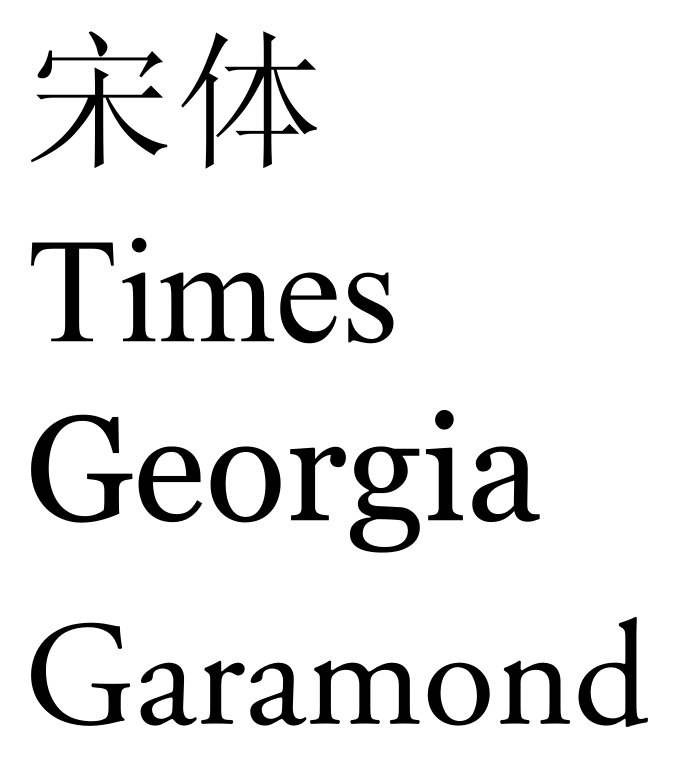
\includegraphics[height=3.5cm]{serif-font.jpg}
      \end{figure}

    特点:{\itshape 正式}
    \end{column}


    \begin{column}{0.5\textwidth}

      非衬线体

      \begin{figure}
        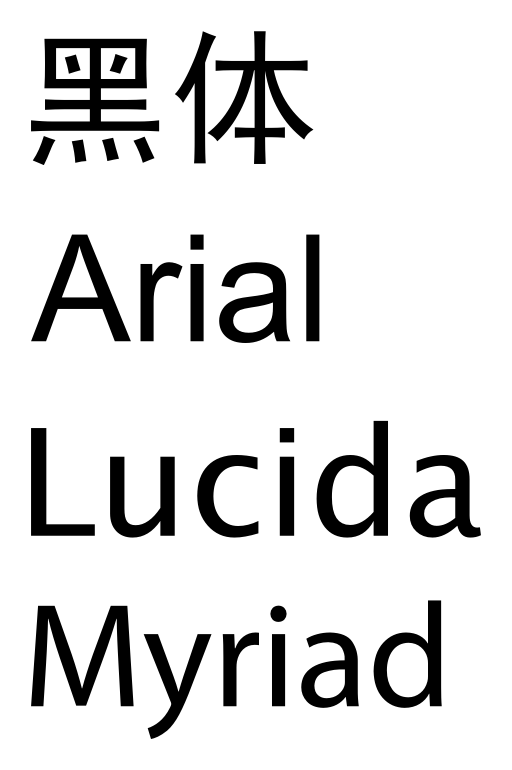
\includegraphics[height=3.5cm]{sans_font.jpg}
      \end{figure}
    特点:{\itshape 时尚}
    \end{column}


  \end{columns}


\end{frame}

\begin{frame}{}
  \begin{figure}
    \includegraphics[width=.8\textwidth]{cbs.jpg}
  \end{figure}
  \begin{figure}
    \includegraphics[width=.8\textwidth]{delta.jpg}
  \end{figure}
\end{frame}

\begin{frame}{}
  
  \begin{figure}
    \includegraphics[width=.8\textwidth]{sprint.jpg}
  \end{figure}
  \begin{figure}
    \includegraphics[width=.8\textwidth]{fedex.jpg}
  \end{figure}

\end{frame}

\section{tips}
\begin{frame}{Notes使用``常用笔''}

  \begin{figure}
    \includegraphics[width=.5\textwidth]{set-pen-style.jpg}
  \end{figure}

  \begin{figure}
    \includegraphics[width=.7\textwidth]{use-pen-style.jpg}
  \end{figure}

\end{frame}

\section{the end}
\begin{frame}

  \begin{block}
    {\itshape
      内容高于形式,文章的版面、字体搞得再漂亮,也不会因此成为《红楼梦》;而《红楼梦》即使是手抄
      本,也依然是不朽的名著。
    }
  \end{block}

  % \begin{block}
  {\itshape
    \begin{itemize}
    \item 好的电视,有电影的味道
    \item 好的数码照片,有胶片的味道
    \item 好的文档,有期刊的味道
    \end{itemize}
  }
  % \end{block}

\end{frame}

\end{document}